\documentclass{article}
\usepackage{tikz}
\usetikzlibrary{arrows.meta, positioning}

\tikzset{
  box/.style={rectangle, draw, fill=gray!10, rounded corners=2pt, minimum width=3cm, minimum height=1cm, align=center},
  smallbox/.style={rectangle, draw, fill=gray!10, rounded corners=2pt, minimum width=3cm, align=center},
  arrow/.style={-Latex}
}

\begin{document}

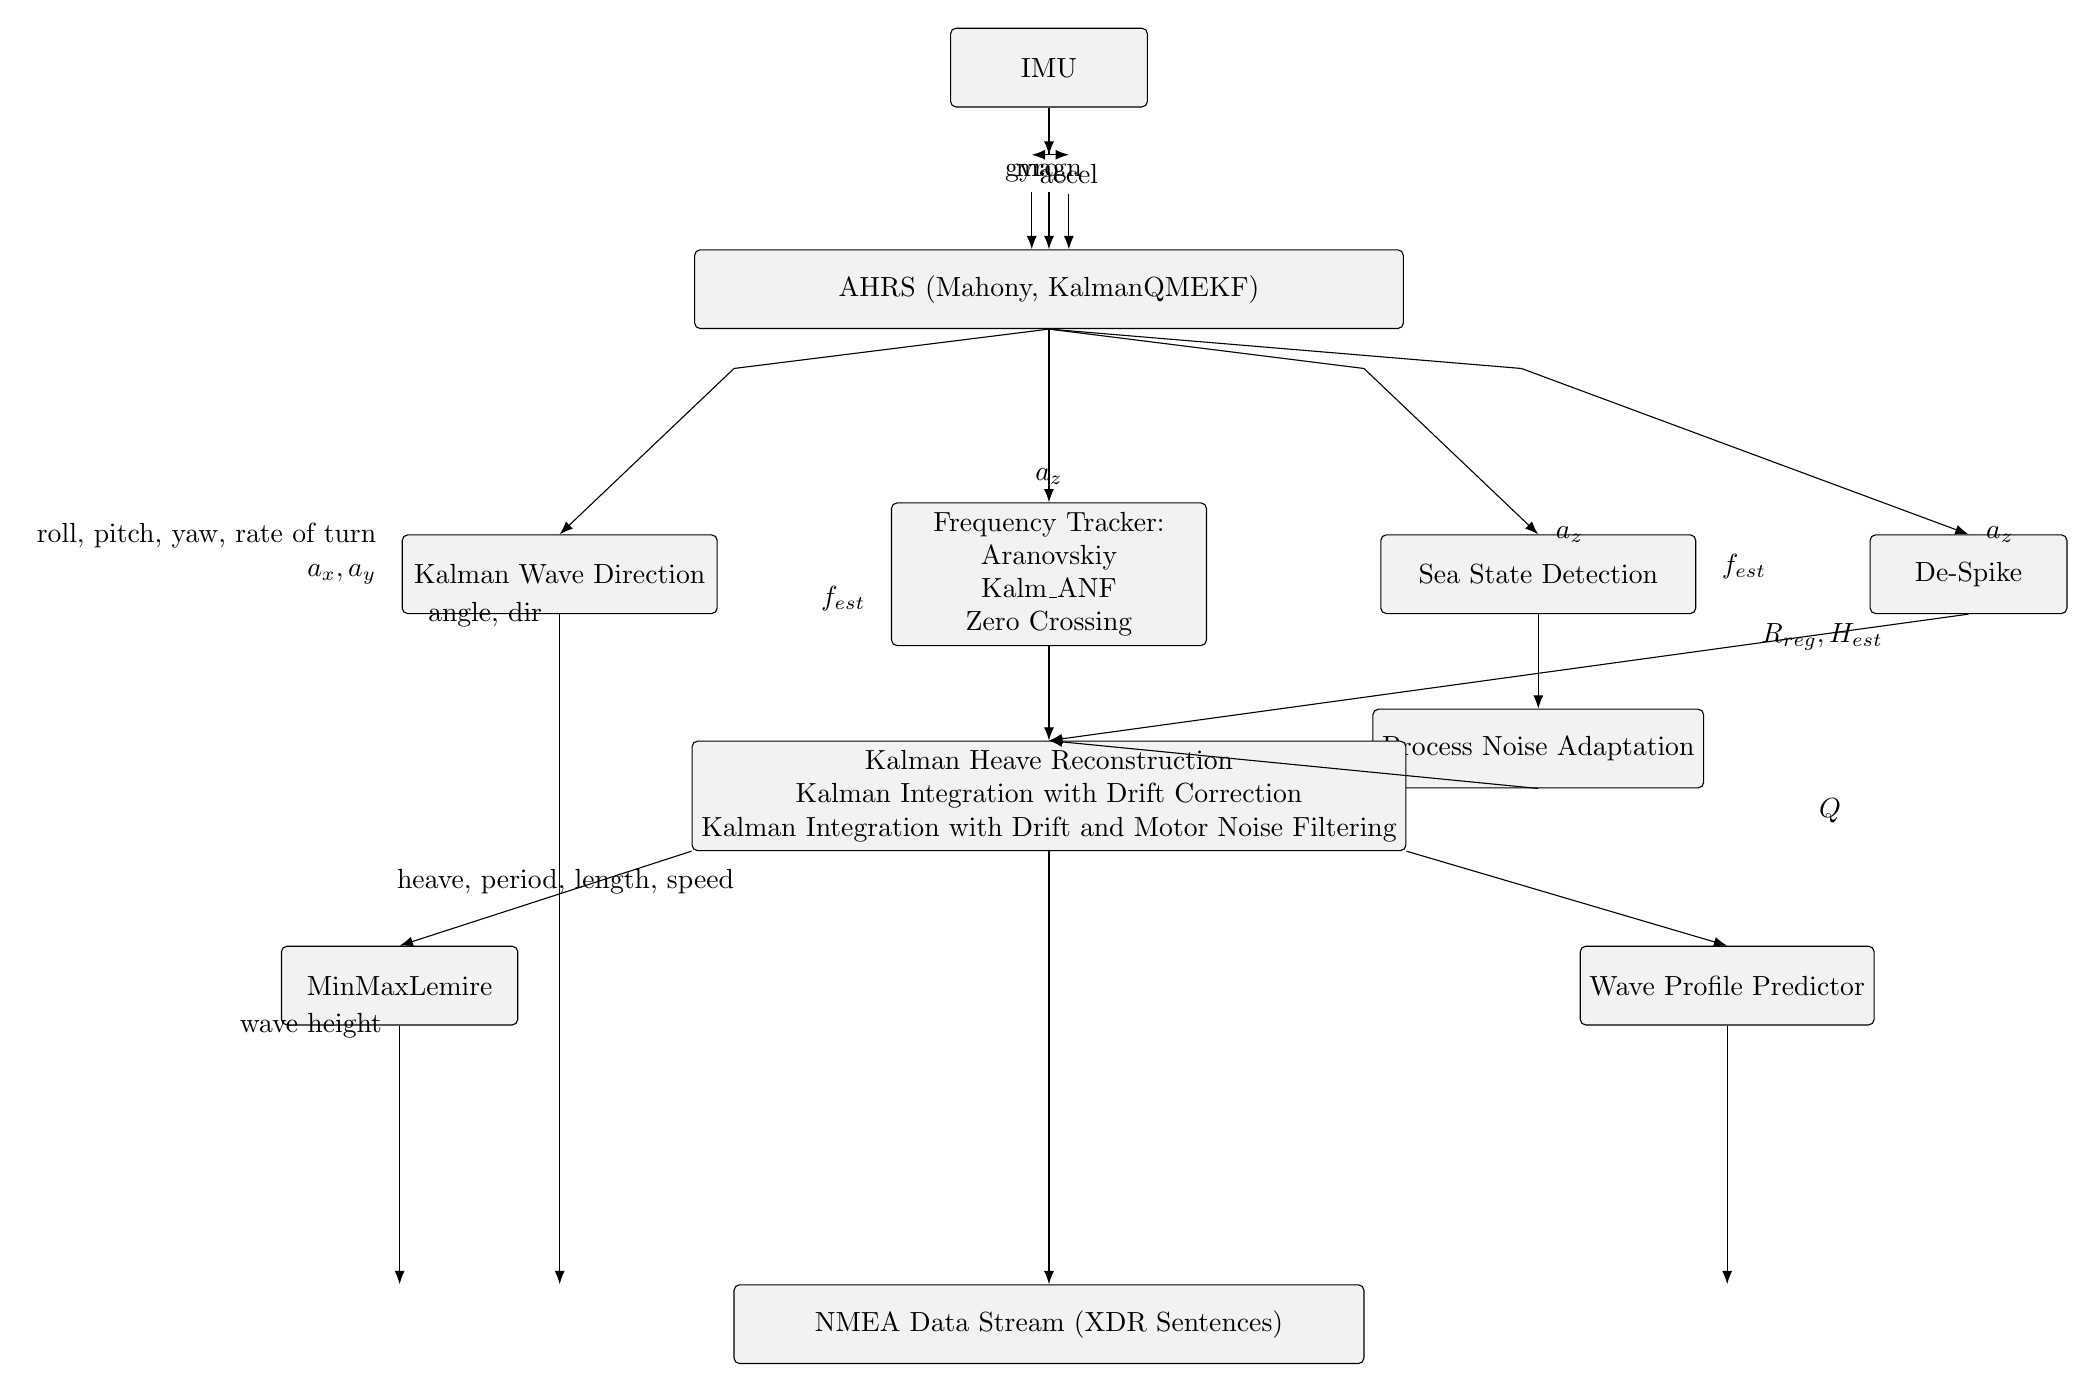
\begin{tikzpicture}[node distance=1.2cm and 2.2cm]

% Top IMU
\node[box, minimum width=2.5cm] (imu) {IMU};

% Sensors
\node[below left=0.6cm and -1.5cm of imu] (gyro) {gyro};
\node[below=0.6cm of imu] (magn) {magn};
\node[below right=0.6cm and -1.5cm of imu] (accel) {accel};

% AHRS
\node[box, below=1.8cm of imu, minimum width=9cm] (ahrs) {AHRS (Mahony, KalmanQMEKF)};

% Connections
\draw[arrow] (imu.south) |- (gyro.north);
\draw[arrow] (imu.south) -- (magn.north);
\draw[arrow] (imu.south) |- (accel.north);
\draw[arrow] (gyro.south) -- (ahrs.north -| gyro.south);
\draw[arrow] (magn.south) -- (ahrs.north -| magn.south);
\draw[arrow] (accel.south) -- (ahrs.north -| accel.south);

% Frequency tracker
\node[box, below=2.2cm of ahrs, minimum width=4cm] (freq) {Frequency Tracker:\\ Aranovskiy\\ Kalm\_ANF\\ Zero Crossing};

% Kalman Wave Direction
\node[box, left=of freq, minimum width=4cm] (wavedir) {Kalman Wave Direction};

% Sea state detection
\node[box, right=of freq, minimum width=4cm] (seastate) {Sea State Detection};

% De-Spike
\node[box, right=of seastate, minimum width=2.5cm] (despike) {De-Spike};

% Process Noise Adaptation
\node[box, below=of seastate, minimum width=3.5cm] (noise) {Process Noise Adaptation};

% Kalman Heave
\node[box, below=of freq, minimum width=8cm] (heave) {Kalman Heave Reconstruction\\ Kalman Integration with Drift Correction\\ Kalman Integration with Drift and Motor Noise Filtering};

% MinMaxLemire
\node[box, below left=of heave, minimum width=3cm] (minmax) {MinMaxLemire};

% Wave profile predictor
\node[box, below right=of heave, minimum width=3cm] (predictor) {Wave Profile Predictor};

% NMEA
\node[box, below=5.5cm of heave, minimum width=8cm] (nmea) {NMEA Data Stream (XDR Sentences)};

% Arrows from AHRS
\draw[arrow] (ahrs.south) -- ++(-4cm, -0.5cm) -- (wavedir.north);
\draw[arrow] (ahrs.south) -- (freq.north);
\draw[arrow] (ahrs.south) -- ++(4cm, -0.5cm) -- (seastate.north);
\draw[arrow] (ahrs.south) -- ++(6cm, -0.5cm) -- (despike.north);

% Arrows downwards
\draw[arrow] (freq.south) -- (heave.north);
\draw[arrow] (wavedir.south) -- (nmea.north -| wavedir.south);
\draw[arrow] (seastate.south) -- (noise.north);
\draw[arrow] (noise.south) -- (heave.north);
\draw[arrow] (despike.south) -- (heave.north);

% Heave outputs
\draw[arrow] (heave.south west) -- (minmax.north);
\draw[arrow] (heave.south east) -- (predictor.north);
\draw[arrow] (heave.south) -- (nmea.north);

% Minmax to NMEA
\draw[arrow] (minmax.south) -- (nmea.north -| minmax.south);
\draw[arrow] (predictor.south) -- (nmea.north -| predictor.south);

% Labels
\node[left=0.2cm of wavedir.west] {${a_x, a_y}$};
\node[left=0.2cm of wavedir.south west, yshift=1.0cm] {roll, pitch, yaw, rate of turn};
\node[above=0.1cm of freq.north] {$a_z$};
\node[right=0.1cm of seastate.north] {$a_z$};
\node[right=0.1cm of despike.north] {$a_z$};
\node[left=0.2cm of freq.south west, yshift=0.6cm] {$f_{est}$};
\node[right=0.2cm of seastate.south east, yshift=0.6cm] {$f_{est}$};
\node[below=0.0cm of noise.south east, xshift=1.6cm] {$Q$};
\node[below=0.0cm of seastate.south east, xshift=1.6cm] {$R_{reg}, H_{est}$};
\node[below=0.1cm of heave.south west, xshift=-1.6cm] {heave, period, length, speed};
\node[left=0.1cm of minmax.south] {wave height};
\node[left=0.1cm of wavedir.south] {angle, dir};

\end{tikzpicture}

\end{document}
